\documentclass[12pt,a4paper]{article}
\usepackage{amsmath,amscd,amsbsy,amssymb,latexsym,url,bm,amsthm}
\usepackage{epsfig,graphicx,subfigure}
\usepackage{enumitem,balance}
\usepackage{wrapfig}
\usepackage{mathrsfs,euscript}
\usepackage[usenames]{xcolor}
\usepackage{hyperref}
\usepackage[vlined,ruled,linesnumbered]{algorithm2e}
\usepackage{array}
\hypersetup{colorlinks=true,linkcolor=black}
\usepackage{float}
\newtheorem{theorem}{Theorem}
\newtheorem{lemma}[theorem]{Lemma}
\newtheorem{proposition}[theorem]{Proposition}
\newtheorem{corollary}[theorem]{Corollary}
\newtheorem{exercise}{Exercise}
\newtheorem*{solution}{Solution}
\newtheorem{definition}{Definition}
\theoremstyle{definition}

\renewcommand{\thefootnote}{\fnsymbol{footnote}}

\newcommand{\postscript}[2]
 {\setlength{\epsfxsize}{#2\hsize}
  \centerline{\epsfbox{#1}}}

\renewcommand{\baselinestretch}{1.0}

\setlength{\oddsidemargin}{-0.365in}
\setlength{\evensidemargin}{-0.365in}
\setlength{\topmargin}{-0.3in}
\setlength{\headheight}{0in}
\setlength{\headsep}{0in}
\setlength{\textheight}{10.1in}
\setlength{\textwidth}{7in}
\makeatletter \renewenvironment{proof}[1][Proof] {\par\pushQED{\qed}\normalfont\topsep6\p@\@plus6\p@\relax\trivlist\item[\hskip\labelsep\bfseries#1\@addpunct{.}]\ignorespaces}{\popQED\endtrivlist\@endpefalse} \makeatother
\makeatletter
\renewenvironment{solution}[1][Solution] {\par\pushQED{\qed}\normalfont\topsep6\p@\@plus6\p@\relax\trivlist\item[\hskip\labelsep\bfseries#1\@addpunct{.}]\ignorespaces}{\popQED\endtrivlist\@endpefalse} \makeatother

\begin{document}
\noindent

%========================================================================
\noindent\framebox[\linewidth]{\shortstack[c]{
\Large{\textbf{Lab08-Graph Exploration}}\vspace{1mm}\\
CS214-Algorithm and Complexity, Xiaofeng Gao \& Lei Wang, Spring 2021.}}
\begin{center}
\footnotesize{\color{red}$*$ If there is any problem, please contact TA Yihao Xie. }

\footnotesize{\color{blue}$*$ Name:Yanjie Ze \quad Student ID:519021910706 \quad Email: zeyanjie@sjtu.edu.cn   }
\end{center}

\begin{enumerate}

	\item Given an undirected graph $G = (V, E)$. Prove the following propositions.
	
		\begin{enumerate}
		\item Let $e$ be a maximum-weight edge on some cycle of connected graph $G=(V,E)$.
		
        Then there is a minimum spanning tree of $G$ that does not include $e$. Moreover, there is no minimum spanning tree of $G$ that includes $e$ if $e$ is the unique maximum-weight edge on the cycle. 
        \begin{proof}
        ~\\
        We prove the first proposition \textbf{by construction}.
        
        Denote a minimum spanning tree as $T$.
        
        If $T$ does not include $e$, this satisfies our requirement.
        
        If $T$ includes $e$: for the cycle including $e$, there must exist an edge not included in the minimum spanning tree $T$, we denote the edge as $e_{cycle}$.Since $e$ is a maximum-weight edge, $e_{cycle}$ may have a smaller weight than $e$ or the same weight as $e$. 
        \begin{itemize}
            \item 
        If $e_{cycle}$ has a smaller weight, $T$ must include $e_{cycle}$ and exclude $e$. Otherwise, $T$ will not be a $MST$. Therefore, this situation is not possible. This means that if $T$ includes $e$, $e$ can't  be the unique maximum-weight edge.
         \item 
        If $e_{cycle}$ has the same weight, we can replace $e$ with $e_{cycle}$. Thus we construct a minimum spanning tree not including $e$, which satisfies our requirement.
      \end{itemize}
      
        Finally, we prove that there is a minimum spanning tree that does not include $e$.
        
        ~\\
        We prove the second proposition \textbf{by contradiction}.
        
        \textbf{Assume} the minimum spanning tree $T$ of the graph $G$ includes the edge $e$, which is an unique maximum-weight edge on some cycle of connected graph $G=(V,E)$.
        
        Since $T$ is a minimum spanning tree, it will have cycles if we add one more edge of the graph $G$.
        
        Since $G$ already has at least one cycle, which we have assumed as the basic setting, we know that: \textbf{for this cycle in the graph, it has at least one edge not included in $\mathbf{T}$.} Otherwise, $T$ will have cycles. Let's denote this edge not included as $e_{cycle}$(in the same cycle with $e$).
        
        By the assumption, $e$ is the unique maximum-weight edge, so $e_{cycle}$ has a smaller weight.
        
        Therefore, \textbf{$\mathbf{T}$ is not a minimum spanning tree}. Because $T$ can remove $e$ and select $e_{cycle}$, which both ensures the connectivity and diminishes the sum of the weights. 
        
        However, this contradicts the assumption, which means the assumption is wrong. So there is no minimum spanning tree including $e$.
        
        By contradiction, we finish proving the second  proposition.
        \end{proof}
		\item Let $T$ and $T'$ are two different minimum spanning trees of $G$. Then $T'$ can be obtained from $T$ by repeatedly substitute one edge in $T\backslash T'$ by one edge in $T'\backslash T$ and meanwhile the result after each substitution is still a minimum spanning tree.
		\begin{proof}
		~\\
		First we introduce \textbf{Lemma 1} and prove it.
		
		\textbf{Lemma 1}: \textit{For two different minimum spanning tree $T,T'$ of $G$, $\forall e \in T\backslash T'$, $\exists e' \in T'\backslash T $, $weight(e)=weight(e')$ and $e,e'$ are in the same cycle of $G$.}
		\begin{proof}
		The relationship of $T$ and $T'$ is shown in Fig.~\ref{set}. The purple part is the intersection of $T$ and $T'$, which we don't care. The white parts are $T\backslash T'$ and $T'\backslash T$, which must exist because $T$ and $T'$ are different.
		
		We randomly pick one edge in $T\backslash T'$ as $e$, and our goal is to find $e'$ in $T'\backslash T$.
		\begin{enumerate}
		    \item 
		$e$ is in a cycle of $G$. Otherwise $e$ will be the necessary edge for both $T$ and $T'$, then $e$ will be in $T\cap T'$.
	
	    \item
	    $T'$ also has an edge in this cycle, different from $e$, denoted as $e'$. If $e'$ is the same with $e$, then $e$ will be in $T\cap T'$. If $T'$ doesn't have an edge in this cycle, $T'$ will lose its connectivity. Therefore, we prove the existence of $e'\in T'\backslash T$.
	    	\item
	    In this cycle, both $e$ and $e'$ can't be the unique maximum-edge, proved by the proposition:\textit{there is no minimum spanning tree of $G$ that includes $e$ if $e$ is the unique maximum-weight edge on the cycle.} 
	    \item
	    Further, in this cycle, $e$ and $e'$ have the same weight. Otherwise, if $e\in T$ has a smaller weight, $T'$ will certainly select $e$ and discard $e'$.
		\end{enumerate}
		Finally, we prove that \textbf{Lemma 1} holds.
		
		\end{proof}
		
		\begin{figure}[H]
		    \centering
		    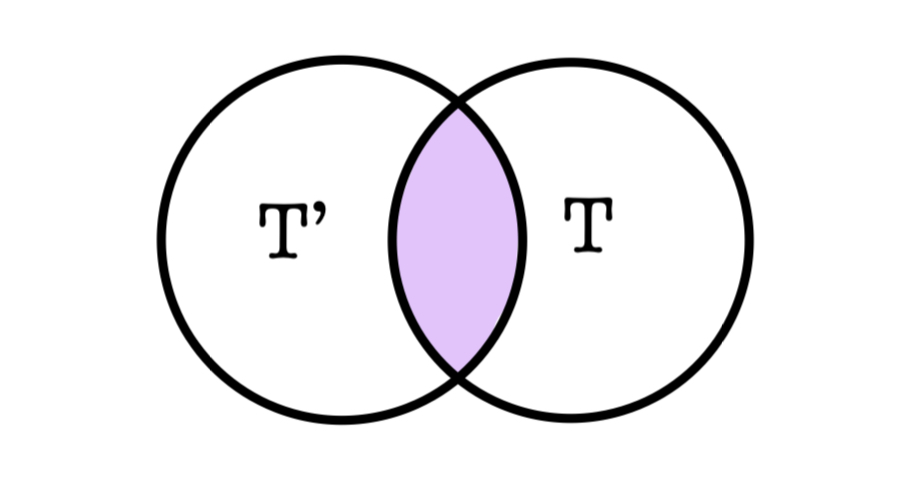
\includegraphics[width=10cm]{set.jpg}
		    \caption{Venn Diagram for MSTs}
		    \label{set}
		\end{figure}
		
		Since \textbf{Lemma 1} holds for both $T$ and $T'$ mutually, this means $|T\backslash T'|$ = $|T' \backslash T|$.
		
		Based on \textbf{Lemma 1}, we are able to repeatedly find an edge $e$ in $T\backslash T'$ and replace it with corresponding $e'$ in $T'\backslash T$, until $T$ is equal to $T'$.
		\end{proof}
		
	\end{enumerate}
	
    \item Let $G=(V,E)$ be a connected, undirected graph. Give an $O(|V|+|E|)$-time algorithm
    to compute a path in $G$ that traverses each edge in $E$ exactly once in each direction. Describe how you can find your way out of a maze if you are given enough coins to apply your algorithm.
    
    \begin{solution}
    ~\\
    Define an array $visit_{vertex}$. If $visit_{vertex}(v)=1$, vertex $v$ has been visited.
    
    Define a matrix $visit_{edge}$. If $visit_{edge}(u,v)=1$, edge $(u,v)$ has been traversed. 
    For convenience, the two variables are set to be global variables.
    
    The \textbf{idea} of the whole algorithm is that \textbf{we modify Depth First Search to not only explore the not visited vertexes, but also explore the not visited edges}.
    
The whole algorithm consists of Alg.~\ref{explore} and Alg.~\ref{DFS}, as shown below.
    
    
    \begin{algorithm}
    \caption{EXPLORE(G,v)}
    \label{explore}
    \textbf{Input:} $G=(V,E)$; $v\in V$; $visit_{vertex}, visit_{edge}$\;
    
    \If{$not\ visit_{vertex}(v)$}
    {
        \Return \;
    }
    \Else{
        $visit_{vertex}(v)=1$\;
    }
    \For{$edge\ (v,u)\in E$}
    {
    \If{$not\ visit_{vertex}(v,u)$}
    {
        $visit_{edge}(v,u)=1$\;
        EXPLORE($G,u$)\;
    }
    }
    
    \end{algorithm}
    
    \textbf{Explanation for Alg.~\ref{explore}}: We do exploration based on whether the edge of one vertex has been visited, since our purpose is to traverse all the edges. 
    
    There exists one case that the old $DFS$ can't solve: Once a vertex has been visited, there may still exist edges not visited. Therefore, we use $visit_{edge}(u,v)$ as our metric to judge whether to explore.
    
    \begin{algorithm}
    \caption{DFS(G)}
    \label{DFS}
    \textbf{Input}: $G=(V,E)$ is a graph\\
    \textbf{Ouput}: $visit_{edge}(u,v)=1, \forall edge(u,v) \in E$\\
    \For{$v\in V$}{$visit_{vertex}(v)=0$\;}
    \For{$edge(u,v)\in E$}{$visit_{edge}(u,v)=0$\;}
    \For{$v\in V$}{
    \If{$not\ visit_{vertex}(v)$}{EXPLORE($G,v$)\;}
    }
    \end{algorithm}
    \end{solution}
    
    Then we embed Alg.~\ref{explore} into \textbf{Depth First Search}, to get Alg.~\ref{DFS}.
    
    
    \textbf{How can we find a way out of maze given enough coins?} 
    
    We can utilize the idea of Alg.~\ref{DFS}.
    \begin{enumerate}
        \item We use the number of coins to represent the times of points we visit.
        \item While we haven't reached the final:
        \begin{enumerate}
            \item We now are at a point.
            \item If the number of coins at this point is equal to the number of available paths, we walk back to the path we come to this point, and go to \textbf{iv}.
            \item Else, Choose one available path that has no coins dropped on it. While we are walking on it, we drop coins to mark it.
            \item Then we reach a new point, and drop a coin on the new point.
        \end{enumerate}
    \end{enumerate}
    
    \item Consider the maze shown in Figure \ref{Fig-Maze}. The black blocks in the figure are blocks that can not be passed through. Suppose the block are explored in the order of right, down, left and up. That is, to go to the next block from $(X,Y)$, we always explore $(X,Y+1)$ first, and then $(X+1,Y)$,$(X,Y-1)$ and$(X-1,Y)$ at last. Answer the following subquestions:
    \begin{enumerate}
        \item Give the sequence of the blocks explored by using DFS to find a path from the "start" to the "finish".
        \begin{solution}
        ~\\
        The sequence of exploring blocks is :
        
        $
        (A,A)(\mathbf{Start})\rightarrow (B,A) \rightarrow (B,B) \rightarrow (B,C) \rightarrow (C,C) (back\ to\  (B,C))\rightarrow (A,C) \rightarrow (A,D)
        $
        $
        \rightarrow (A,E) \rightarrow (B,E) \rightarrow (C,E) \rightarrow (D,E) \rightarrow (D,D)(\mathbf{Finish})
        $
~\\

        Then the path from the start to the end is the following sequence, which is shown in Fig.~\ref{maze1}:
        
        $
        (A,A)(\mathbf{Start})\rightarrow (B,A) \rightarrow (B,B) \rightarrow (B,C) \rightarrow (A,C) \rightarrow (A,D)\rightarrow (A,E) \rightarrow (B,E) \rightarrow (C,E) \rightarrow (D,E) \rightarrow (D,D)(\mathbf{Finish})
        $
        
        \end{solution}
        
        \item Give the sequence of the blocks explored by using BFS to find the \underline{shortest} path from the "start" to the "finish".
        \begin{solution}
        ~\\
        The sequence of exploring blocks is:
        
        $
        (A,A)(\mathbf{Start}) \rightarrow (B,A) \rightarrow (B,B) \rightarrow (C,A) \rightarrow (B,C) \rightarrow (D,A) \rightarrow (C,C) \rightarrow (A,C) \rightarrow (D,B) \rightarrow (A,D) \rightarrow (E,B) \rightarrow (A,E) \rightarrow (E,C) \rightarrow (B,E) \rightarrow (E,D) \rightarrow (C,E) \rightarrow (D,D)(\mathbf{1st\ path\ reaches\ the\ final.}) \rightarrow (D,E) \rightarrow (D,D)(\mathbf{2nd\ path\ reaches\ the\ final})
        $
        
        ~\\
        There exist two paths in total, and the shortest path is the following sequence, as shown in Fig.~\ref{maze2}:
        
        $
        (A,A)(\mathbf{Start}) \rightarrow (B,A) \rightarrow (C,A) \rightarrow (D,A) \rightarrow (D,B) \rightarrow (E,B) \rightarrow (E,C) \rightarrow (E,D) \rightarrow (D,D)(\mathbf{Finish})
        $
        
        \begin{figure}[htbp]
            \centering
            \begin{minipage}[t]{0.48\textwidth}
            \centering
            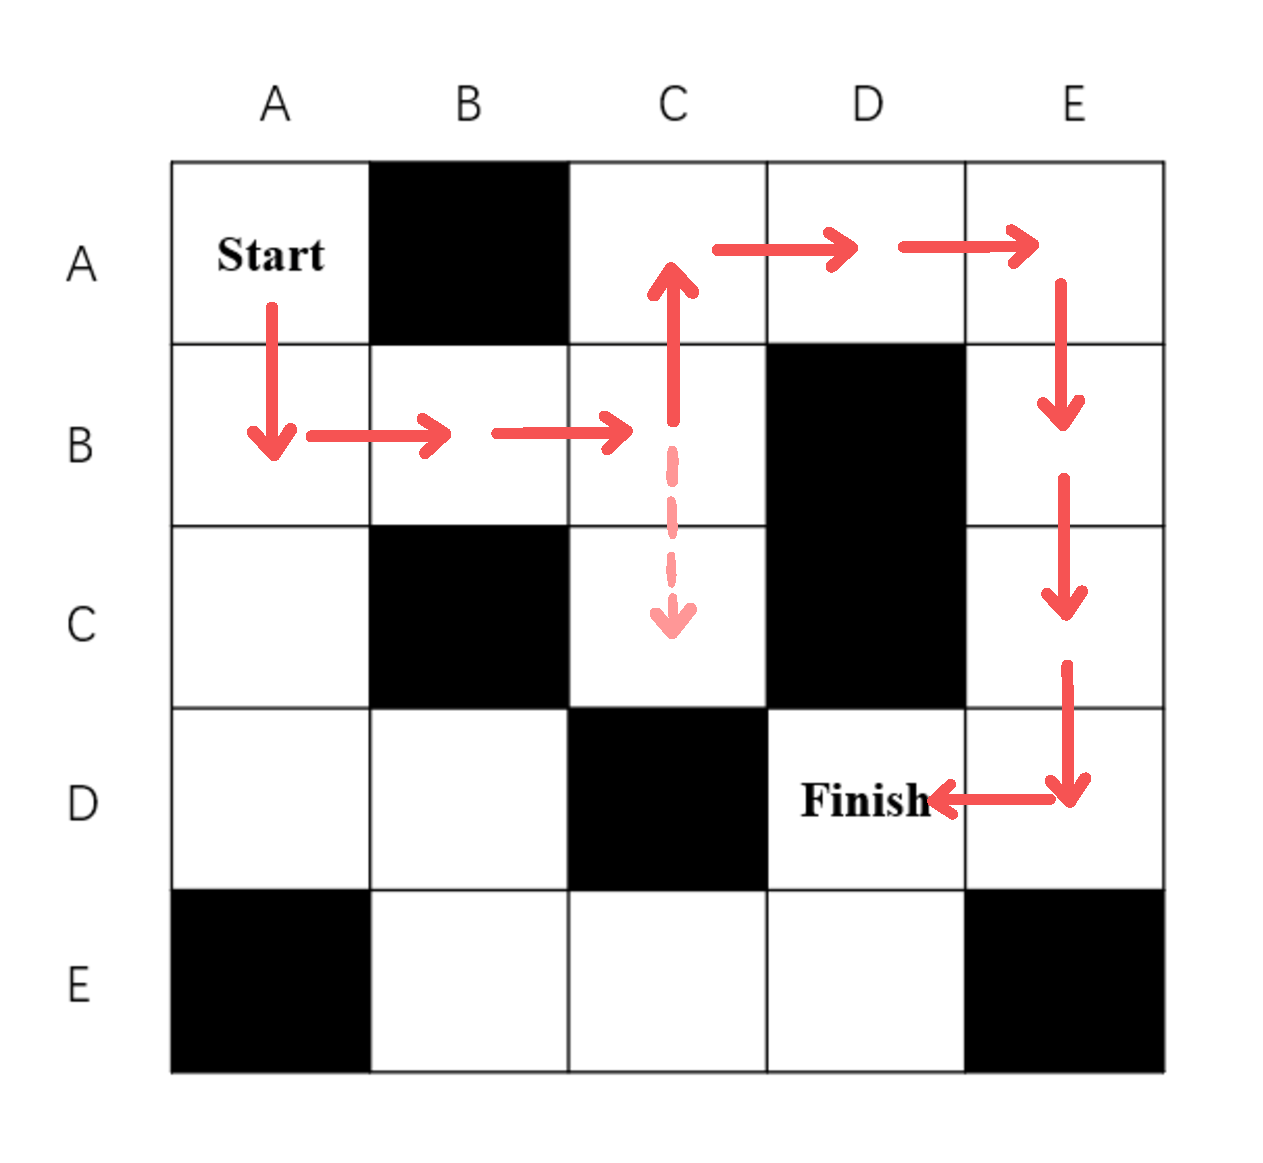
\includegraphics[width=6cm]{maze1.pdf}
            \caption{Maze Path by DFS}\label{maze1}
            \end{minipage}
            \begin{minipage}[t]{0.48\textwidth}
            \centering
            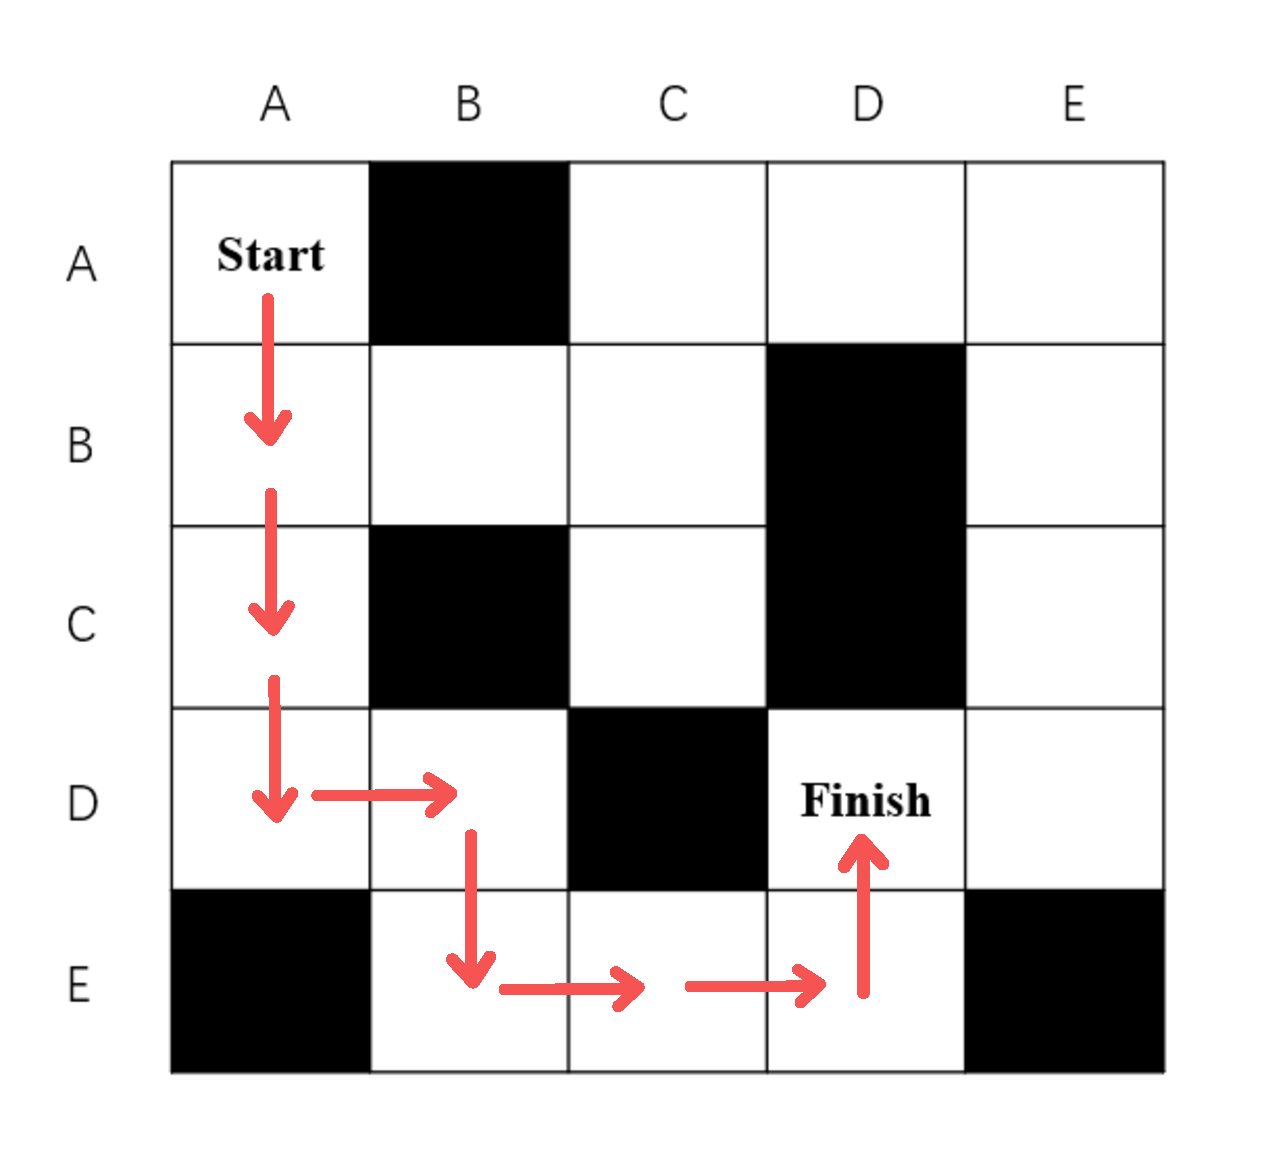
\includegraphics[width=6cm]{maze2.pdf}
            \caption{Shortest Path by BFS}\label{maze2}
            \end{minipage}
            \end{figure}
        \end{solution}
        \item Consider a maze with a larger size. Discuss which of BFS and DFS will be used to find one path and which will be used to find the shortest path from the start block to the finish block.
        \begin{solution}
        \textbf{DFS is used to find one path.} 
        
        $DFS$ will go deeper and deeper when there still exists an available path in front of it. Once $DFS$ has reached the destination, it will stop and not explore other possible path(in this problem). Although in the worst case $DFS$ will go through all the paths and finally get one available path, using $DFS$ to find a path is still a gooc choice.
        
        \textbf{BFS is used to find the shortest path.}
        $BFS$ will go through all possible paths. In the end we compare all possible paths and get the shortest path. 
        \end{solution}
    \end{enumerate}
    
    \begin{figure}[!htbp]
	\centering
	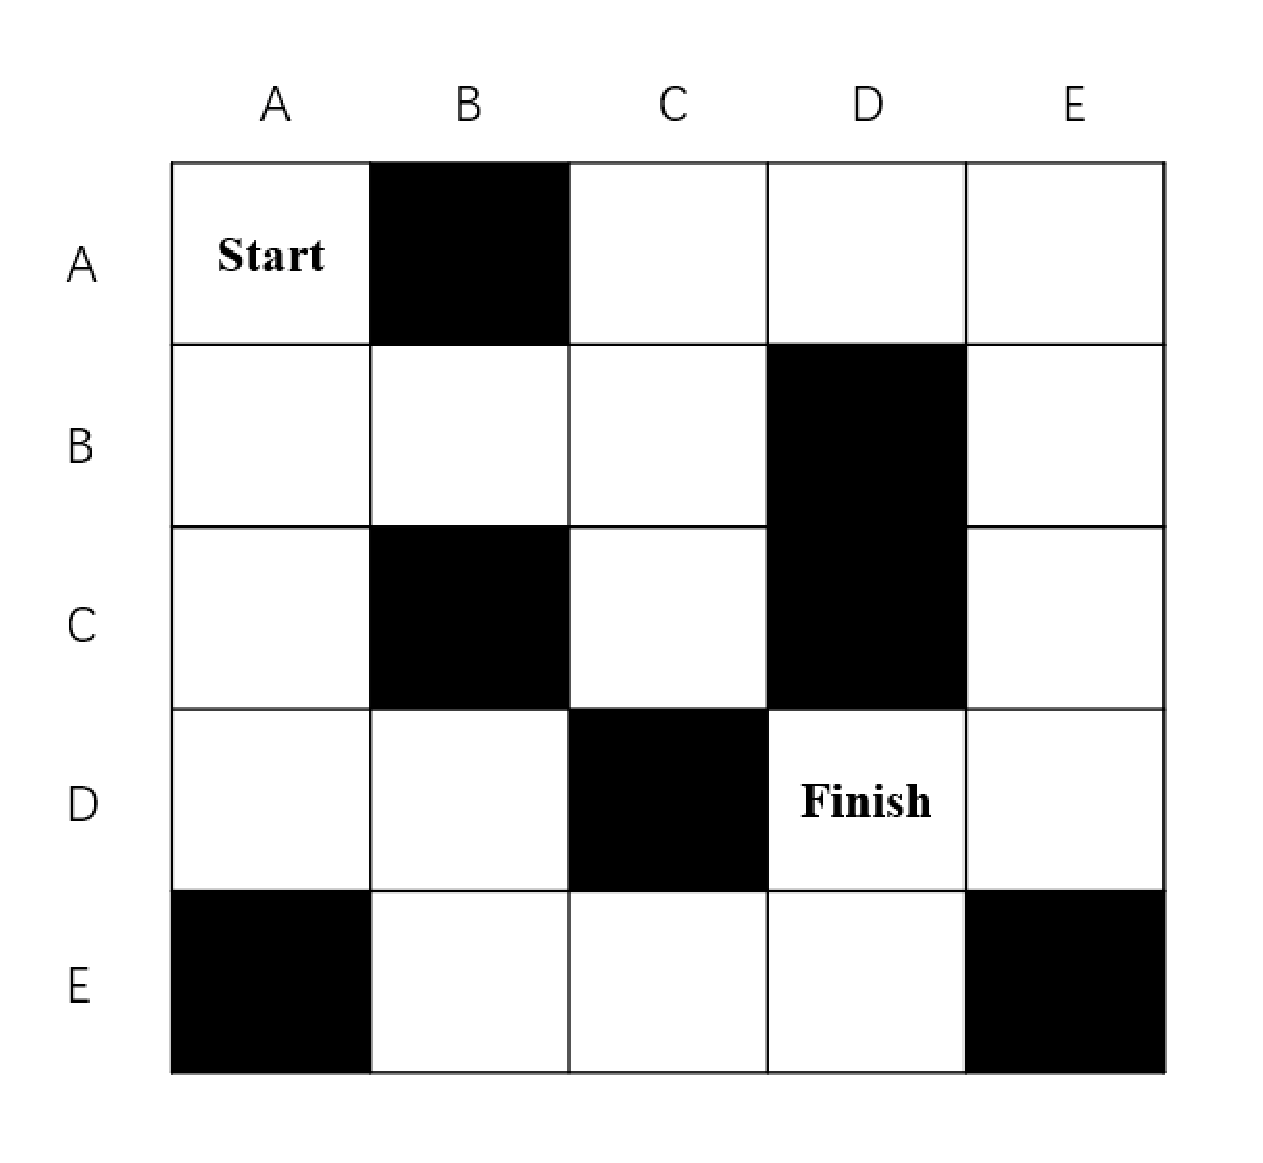
\includegraphics[width=6cm]{Fig-Maze.pdf}
	\caption{An example of making room for one new element in the set of arrays.}
	\label{Fig-Maze}
	\end{figure}
 	
	\item Given a directed graph $G$, whose vertices and edges information are introduced in data file "SCC.in". Please find its number of Strongly Connected Components with respect to the following subquestions.
    
    \begin{enumerate}
    	\item Read the code and explanations of the provided C/C++ source code "SCC.cpp", and try to complete this implementation.
    	\begin{solution}
    	~\\
    	The full code is in \textbf{SCC.cpp}. And the number of Strongly Connected Components is \textbf{202}.
    	
    	In the program, we implement the algorithm following these steps:
    	~\\
    	
    	\textbf{Program. SCC Counting}
    	\begin{enumerate}
    	    \item Construct an adjacent matrix $10000\times 10000$ based on edges, to represent the graph.
    	    \item Reverse the matrix.
    	    \item Run \textbf{Depth-first Search} on the matrix and get the post number of each vertex.
    	    \item Reverse the matrix.
    	    \item Initialize $num_{components}=0$.
    	    \item While the graph is not empty:
    	    \begin{enumerate}
    	        \item Find the vertex with the largest post number.
    	        \item Run DFS starting from this vertex to delete the vertexes in this SCC.
    	        \item $num_{components} = num_{components}+1$
    	    \end{enumerate}
    	    \item Return the number of SCC $num_{components}$.
      	\end{enumerate}
    	\end{solution}
    	\item Visualize the above selected Strongly Connected Components for this graph $G$. Use the $Gephi$ or other software you preferred to draw the graph. {\color{blue}(If you feel that the data provided in ``SCC.in'' is not beautiful, you can also generate your own data with more vertices and edges than $G$ and draw an additional graph. Notice that results of your visualization will be taken into the consideration of Best Lab.)}
    	\begin{solution}
    	The visualization of Strongly Connected Components is shown in Fig.~\ref{scc}, supported by \textit{Gephi}. The larger the component in the graph is, the more vertexes it includes.
    	 \begin{figure}[H]
    	    \centering
    	    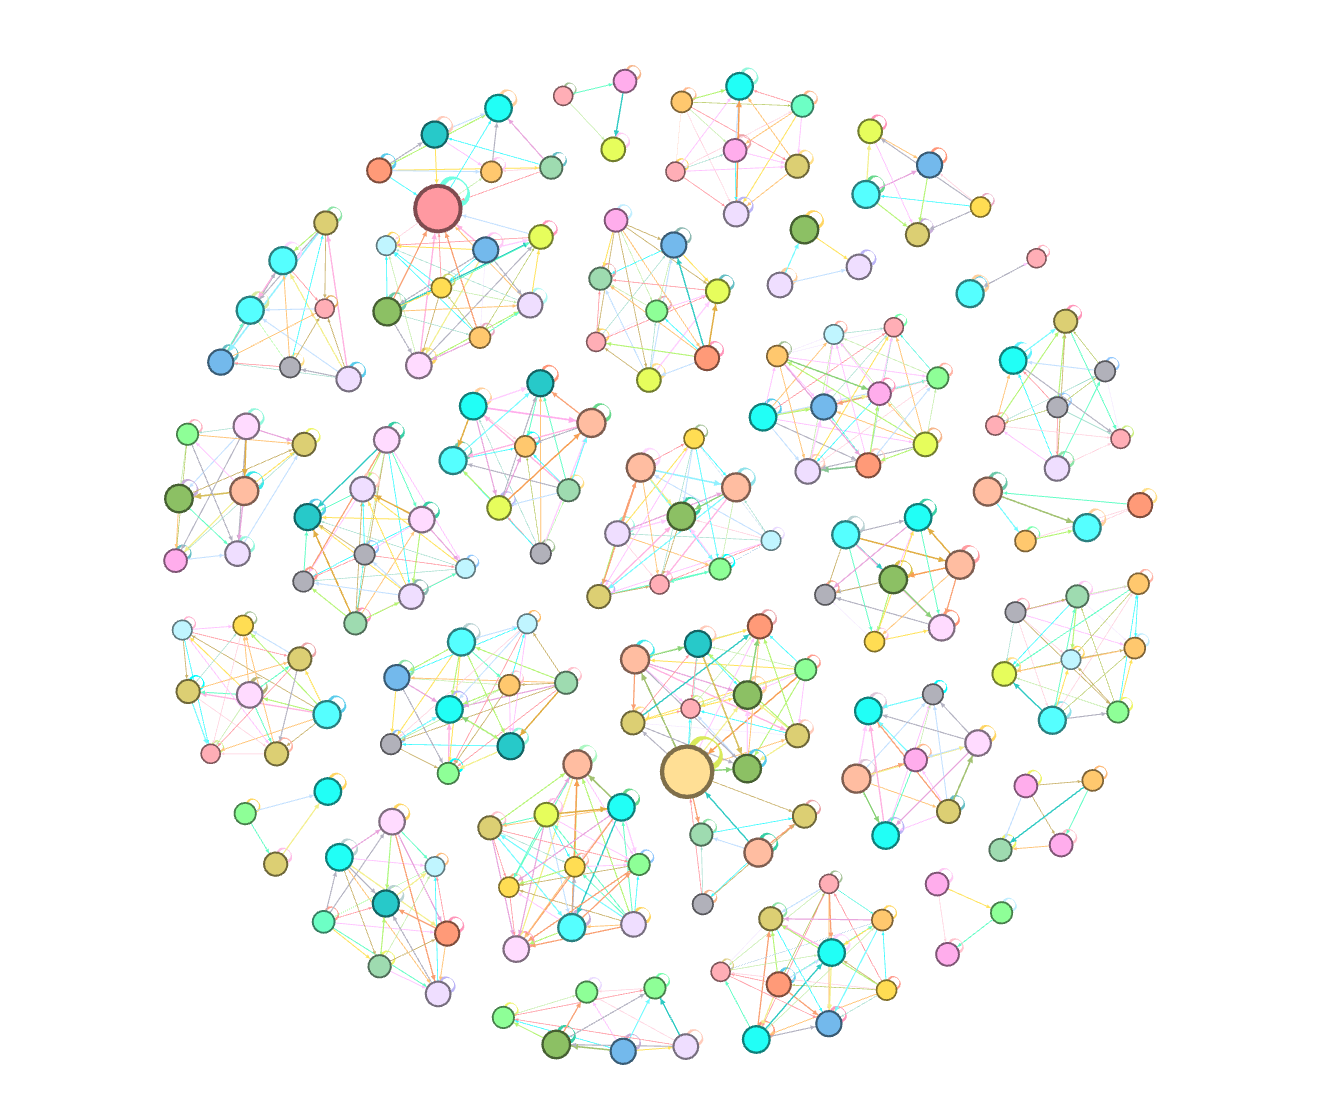
\includegraphics[width=0.8\textwidth]{graph.png}
    	    \caption{SCC Graph}
    	    \label{scc}
    	\end{figure}
    	\end{solution}
 	
    \end{enumerate}	
\end{enumerate}

	  

\textbf{Remark:} Please include your .pdf, .tex, .cpp files for uploading with standard file names.
\newpage


%========================================================================
\end{document}